\scanpage{20}
\mspage{18}
$\underline{R}f_*(\underline{\Omega}^{\bullet}_{X/S})$, considéré comme objet de la catégorie dérivée $D(\underline{O}_S)$. A vrai dire, je n'ai pas vérifié pour cette connexion une condition de ``nullité de la \deleted{\unsure{torsion}} \inserted{courbure}''; c'est \deleted{vrai} vérifié en tous cas (par voie transcendante !) si $S$ est lisse, sur $R$ réduit de caractéristique nulle. [Il faut noter d'ailleurs qu'il n'y a pas d'espoir de montrer que la connexion en question provient toujours d'une stratification: c'est \uline{faux} en caractéristique $p>0$; la raison étant que la cohomologie de De Rham pour une variété algébrique non complète (par exemple affine) n'est plus du tout raisonnable, étant beaucoup trop grosse. Pour pouvoir espérer une stratification sur $\underline{R}f_*(\underline{\Omega}^{\bullet}_{X/S})$, sans restriction de caractéristique, il faut donc supposer $f$ \uline{propre}.]

c) La nécessité d'une interprétation cristallographique de la cohomologie de De Rham est également suggérée par le problème que j'avais signalé dans mon papier bleu sur De Rham: si $R$ est le spectre du corps des complexes, $S$ lisse sur $R$ et $X$ lisse et propre sur $S$, alors la théorie transcendante de la cohomologie nous fournit une suite spectrale $H^p(S^{\mathrm{an}},R^qf^{\mathrm{an}}_*(\underline{C}_{S^{\mathrm{an}}}))\Longrightarrow H^{\bullet}(X^{\mathrm{an}},\underline{C})$, dont le terme initial et l'aboutissement d'autre part ont une description purement algébrique, comme cohomologie de De Rham de $X$, et de $S$ à coefficients dans les $\underline{R}^qf_*(\underline{\Omega}^{\bullet}_{X/S})$ \uline{munis de leur connexion canonique} \inserted{\uline{intégrable}} (ce qui permet de les prendre comme coefficients dans la cohomologie de De Rham). On aimerait trouver une interprétation purement algébrique de cette suite spectrale toute entière.

2.2. Je vais préciser \deleted{\unsure{un genre d'énoncé précis}} l'affirmation du titre, en me plaçant \figure{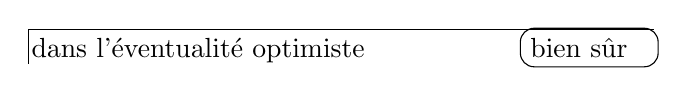
\begin{tikzpicture}[baseline=(a.base)]
\node[anchor=base west,inner sep=1pt] (a) at (0,0) {dans l'éventualité optimiste};
\node[anchor=base west,inner sep=2pt] (b) at (6.3,0) {bien sûr};
\draw (0,-0.08)--(0,0.35)--(7.95,0.35);
\draw[rounded corners=5pt] (6.25,-0.12) rectangle (8,0.37);
\end{tikzpicture}} où on n'aurait pas besoin de s'isogéniser.
\deleted{On \deleted{veut} désigne, pour abréger, par le mot ``\uline{complexe}'' \unsure{sur} un préschéma $S$, un complexe de Modules à cohomologie quasi-cohérente, considéré comme objet de la catégorie dérivée qu'on sait; Les catégories de ces complexes, pour une base variable,}
Comme les cristaux de modules sur un préschéma $S$ forment une catégorie abélienne, on peut prendre la catégorie dérivée; ses objets seront appelés simplement ``complexes de cristaux''. Un tel animal induit sur $S$, et plus généralement sur tout objet-but $T$ d'un objet $(U\longrightarrow T)$ du site cristal-
\margin{19}
